\documentclass{article}
\usepackage{listings}
\usepackage{amsmath}
\usepackage{graphicx}

\begin{document}

\title{MAT362 - Project 3 Report}
\author{Christopher D. Whitney}

\maketitle

\section*{Introduction}
The goal of this project is to (1) code, test, and compare Euler’s and Runge-Kutta methods for solving first order initial value problems, (2) to apply the Runge-Kutta solver toward solving systems of first order initial value problems and (3) use these solvers to code and test the "shooting method" to find a solution(s) to boundary value problems.

The report will be structured as follows, first we will explain the algorithms and then we will walk through each of the problems outlined in the description of the project.

\section*{Overview of Algorithms}
In the following section we will desribe the key algorthims used in this project, which are Eulers method, the Runge-Kutta method and the "shooters method" which uses, in our cases, the Runge-Kuttaa.

\subsection*{Eulers Method}
Euler's method is a direct numerical method used to approximate ordinary differential equations (ODE) equations given an initial value. It works by iterating over a given number of steps, thus it is a direct method. It usses this idea of local linearity  to create small line segments and join them together to obtain an approximate the solution to the ODE. 
 
\subsection*{Rung-Kutta Method}
Rung-Kutta method is similar to Euler's method is the fact that it a direct method. However, it uses the idea of weighted intermediate slopes to more accurately approximate the next time-step. 

\subsection*{"Shooters Method"}
The "Shooter method" uses the Rutta-Kutta method described above and is used to find solution to bounder value problems. It works by iterating over a number of guess for the bound and solves the given equation given those bounds and then repeats. This is also a direct method because the number of guess it determined a head of time. 

\section*{Part A}
\subsection*{(a)}
$$ \text{5.1.1 a  } y(t) = e^{sin(t)} $$
$$ \text{5.1.1 b  } y(t) = t^2 (e^t - e)$$
$$ \text{5.1.1 c  } y(t) = \frac{t^4 e^t - 4t^3e^t + 12t^2e^t − 24te^t + 24e^t + (\sqrt{2} - 9)e}{t^2}$$
$$ \text{5.1.1 d  } y(t) = 1 + t^4$$
$$ \text{5.1.2 a  } y(t) = ln(e^t - 1 + e) $$
$$ \text{5.1.2 b  } y(t) = \frac{-cos(2t)+cos(2) + 4}{2t^2}$$
$$ \text{5.1.2 c  } y(t) = e^{-t}(e^{t/2}(t-2)  + \sqrt{2} e)^2$$
$$ \text{5.1.2 d  } y + ln(y) = t + ln(t)$$

\subsection*{(b)}
Running Euler method on each of the above functions, the red line is the exact solution and the blue is the approximate solutions with $ n \in \{ 10, 20, 40, 80, 160 \}$. 

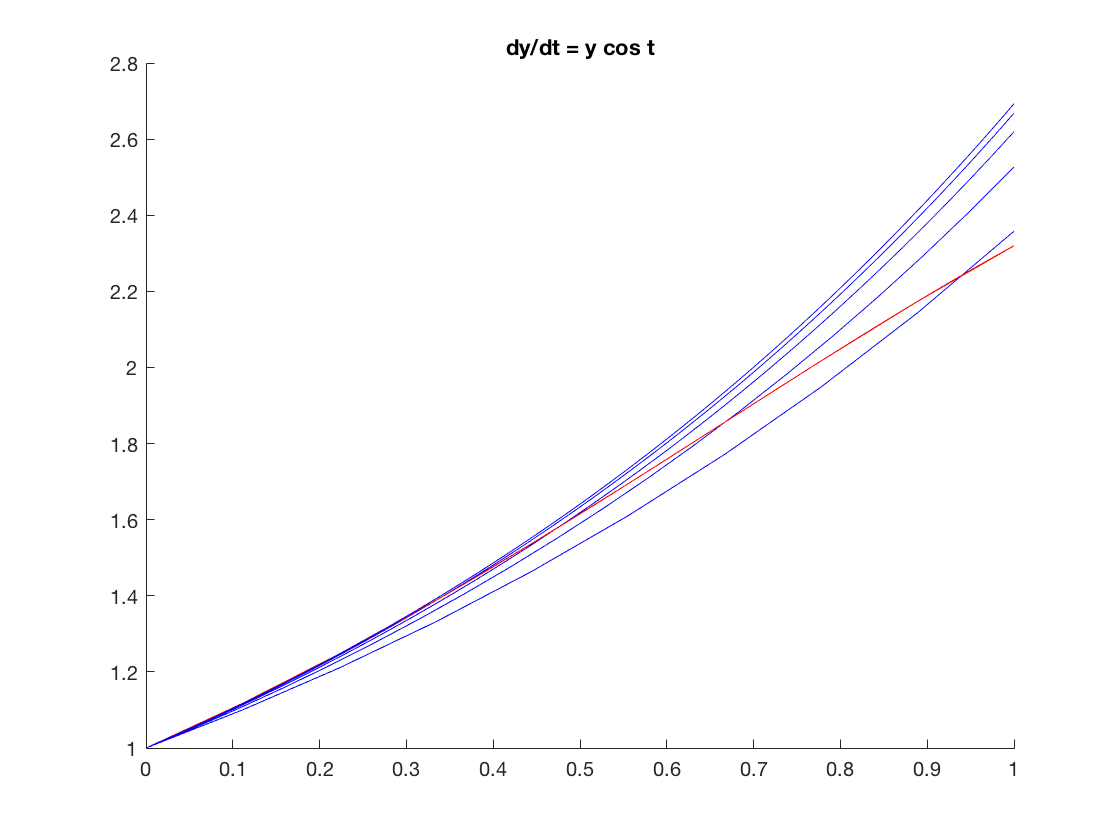
\includegraphics[height=8cm]{parta_1}\\
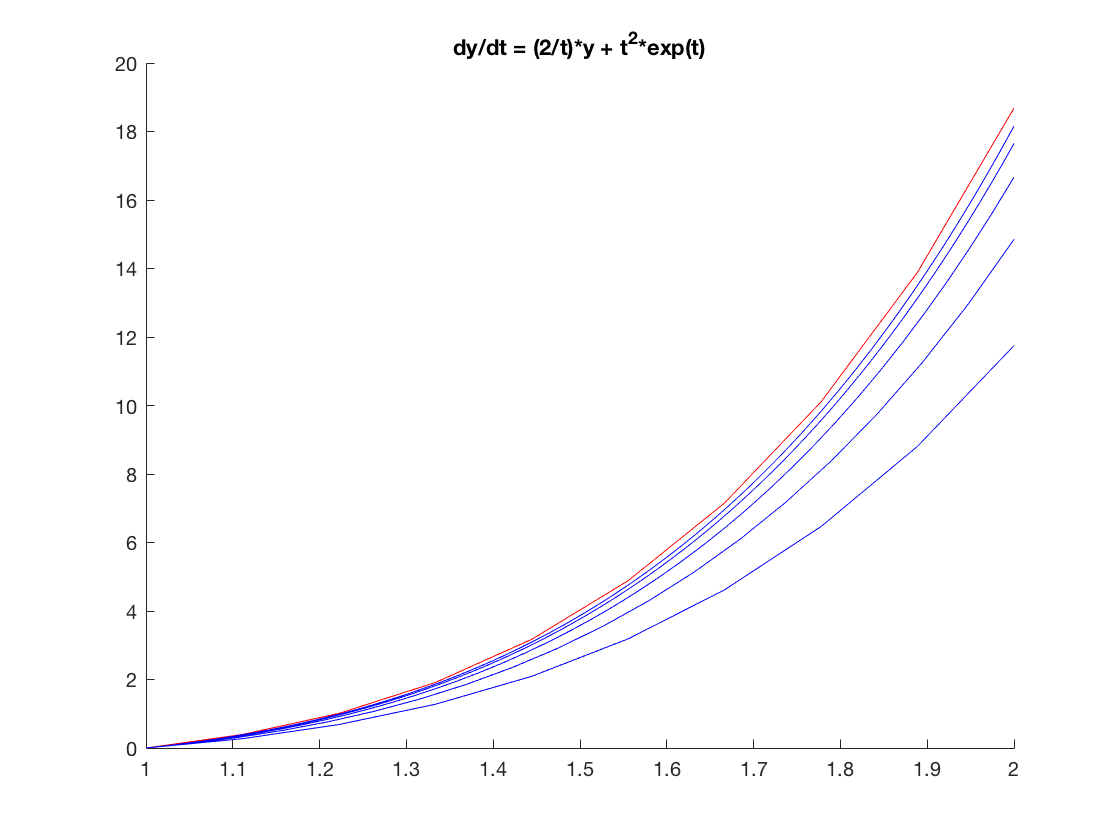
\includegraphics[height=8cm]{parta_2}\\
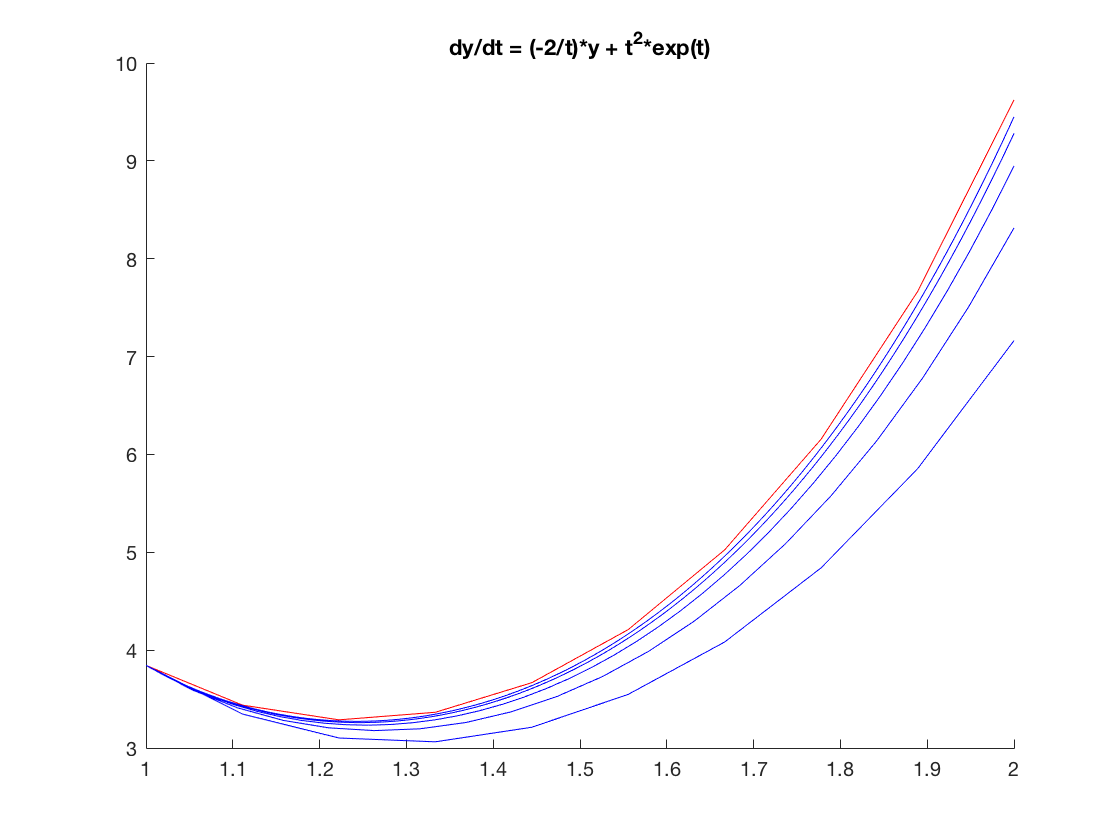
\includegraphics[height=8cm]{parta_3}\\
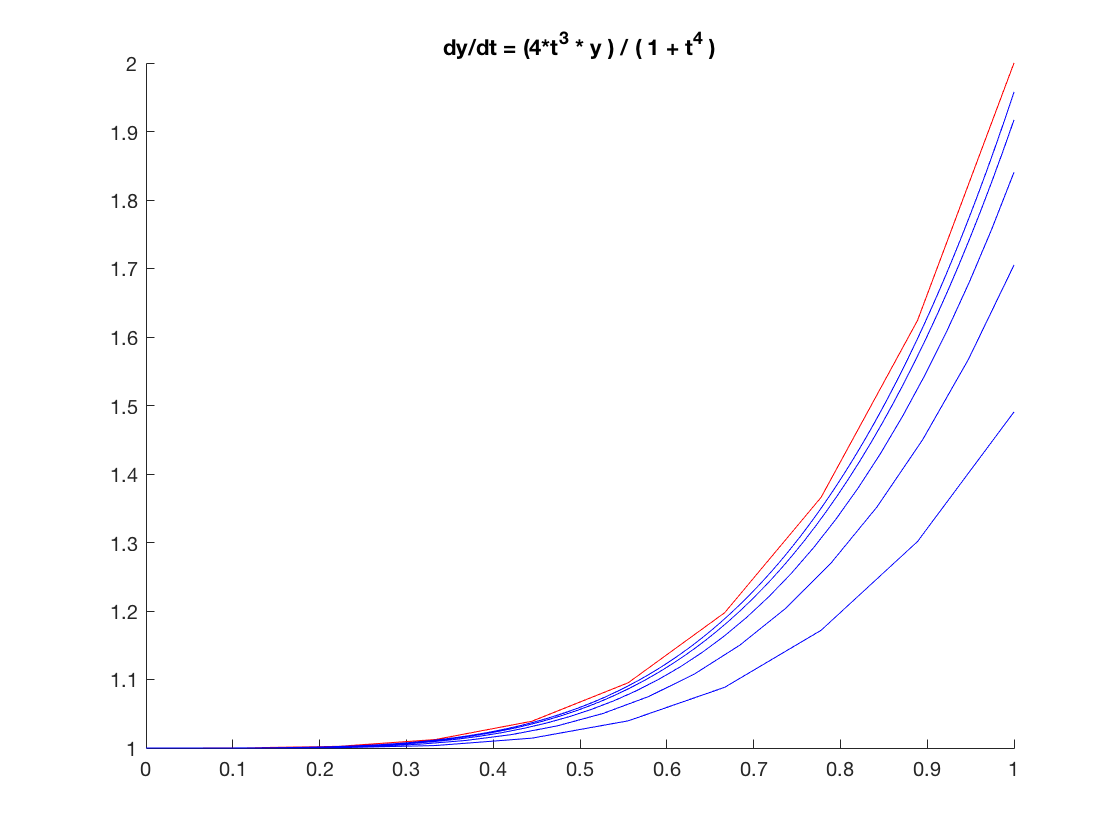
\includegraphics[height=8cm]{parta_4}\\
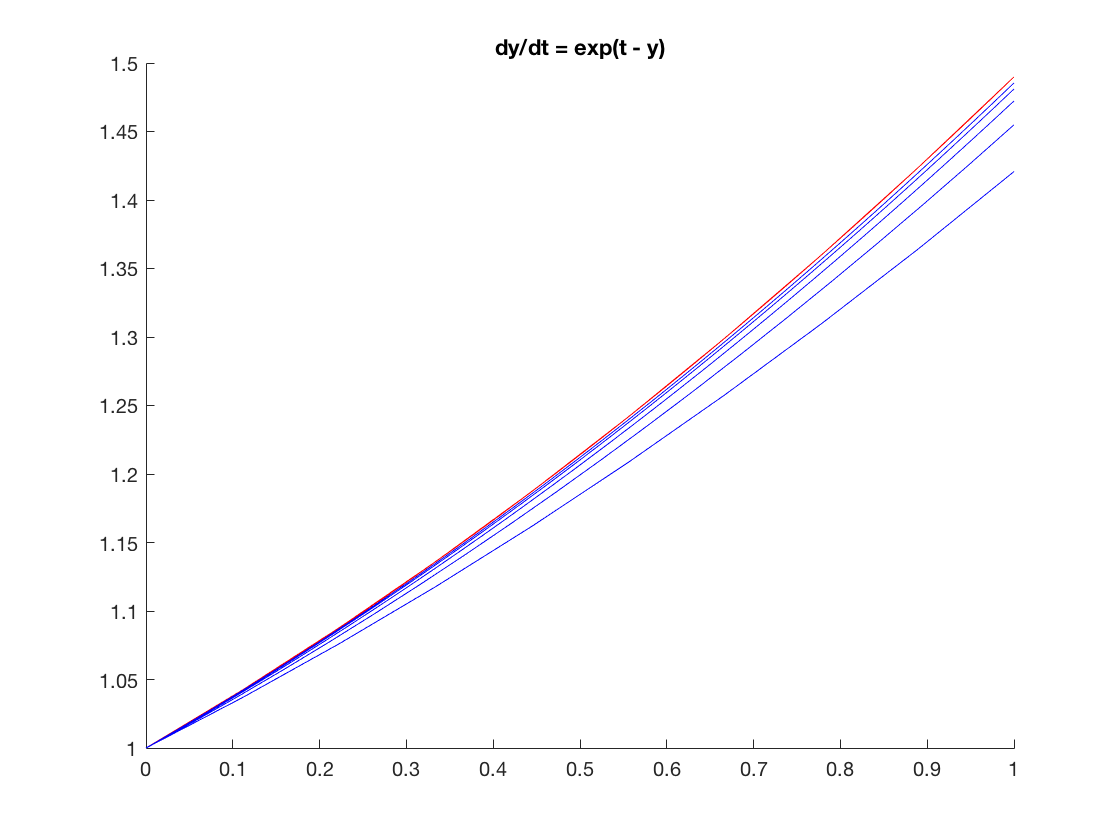
\includegraphics[height=8cm]{parta_5}\\
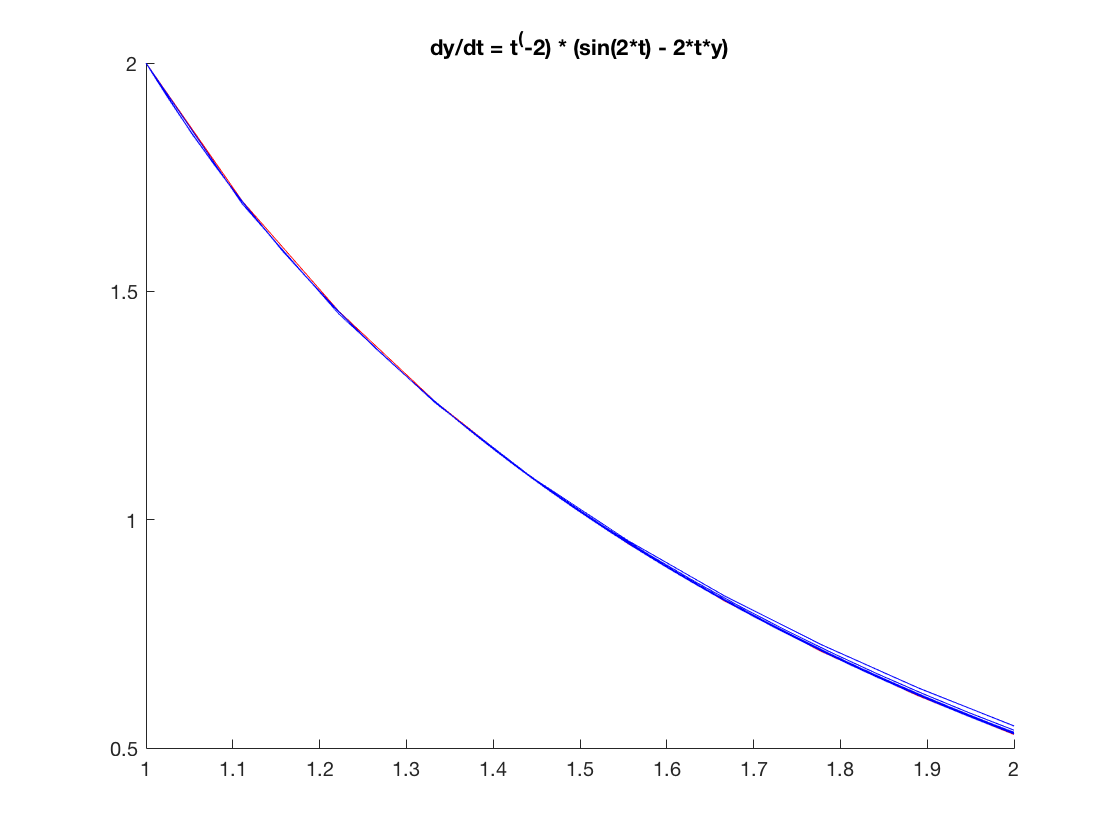
\includegraphics[height=8cm]{parta_6}\\
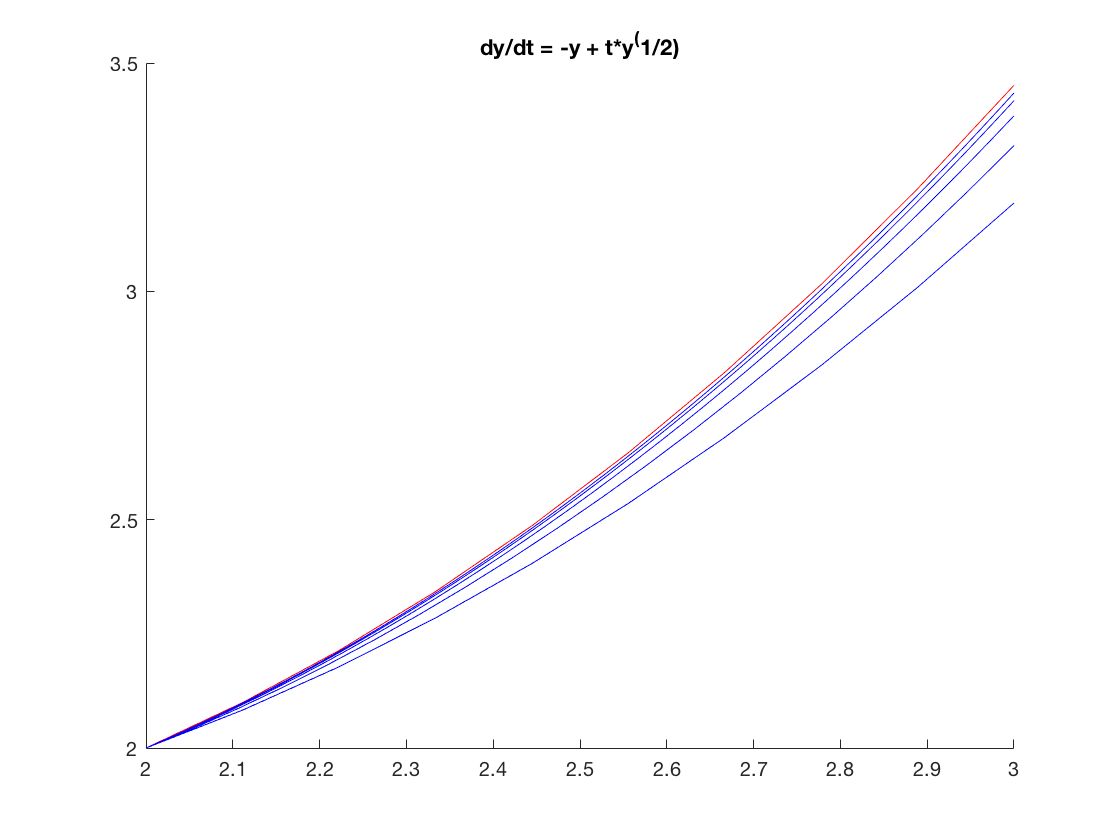
\includegraphics[height=8cm]{parta_7}\\


\subsection*{(c)}
Running Runge-Kutta methods on each of the above functions, the red line is the exact solution and the blue is the approximate solutions with $ n \in \{ 10, 20, 40, 80, 160 \}$. 

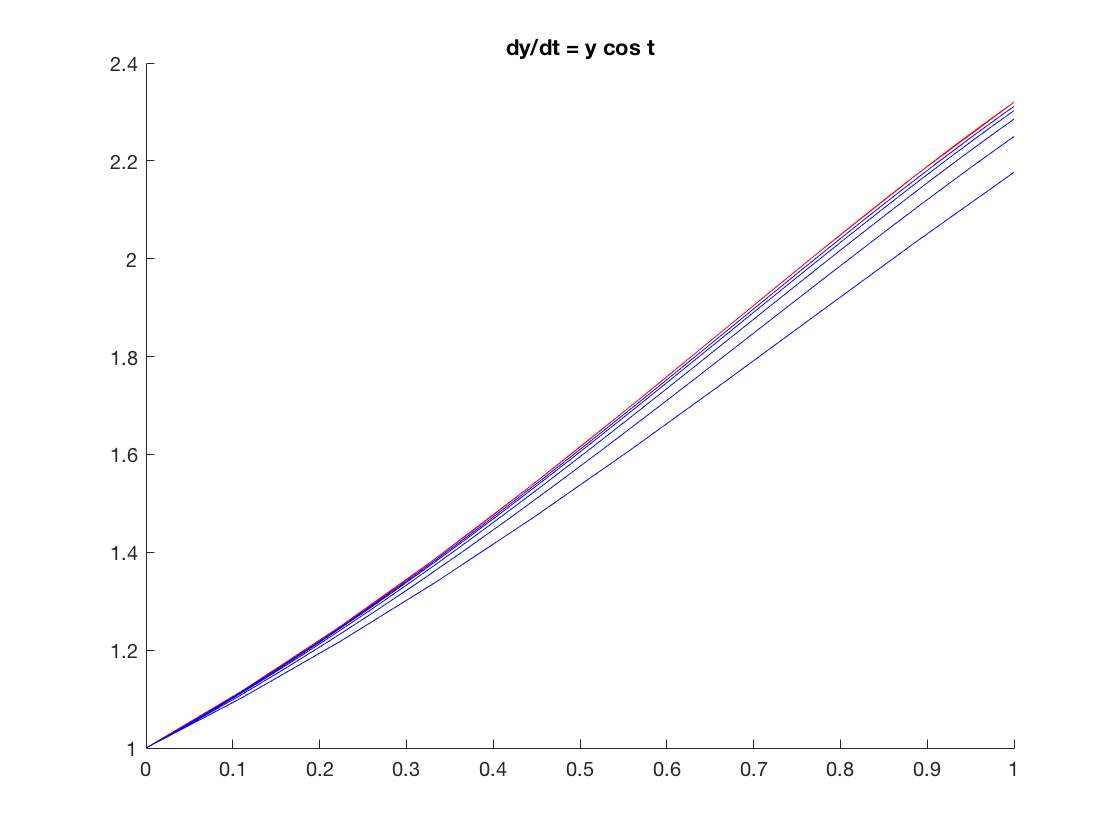
\includegraphics[height=8cm]{partc_1}\\
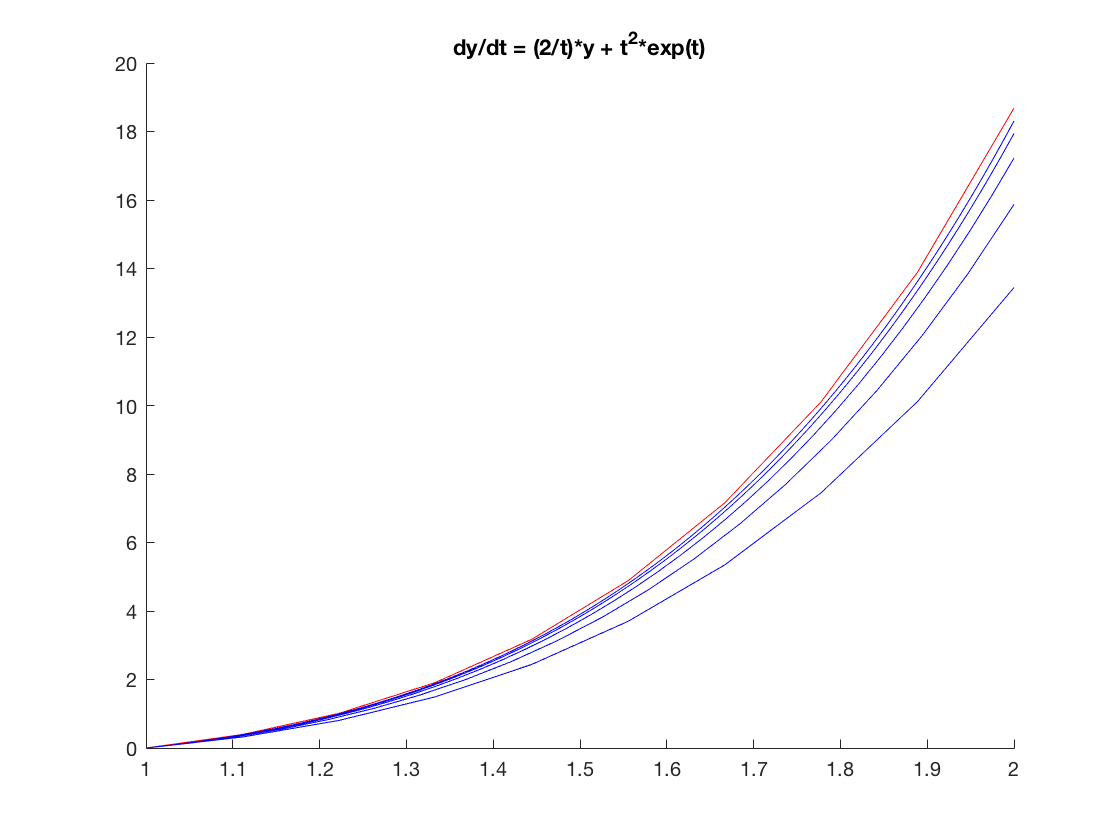
\includegraphics[height=8cm]{partc_2}\\
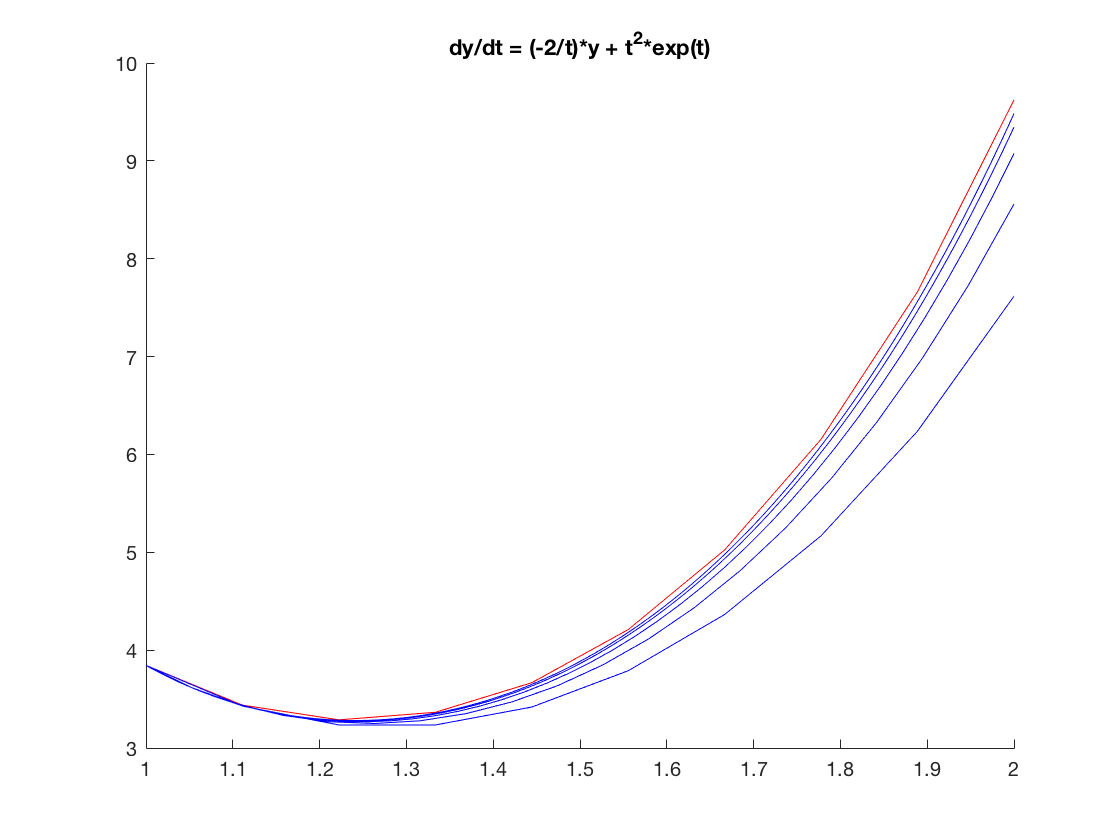
\includegraphics[height=8cm]{partc_3}\\
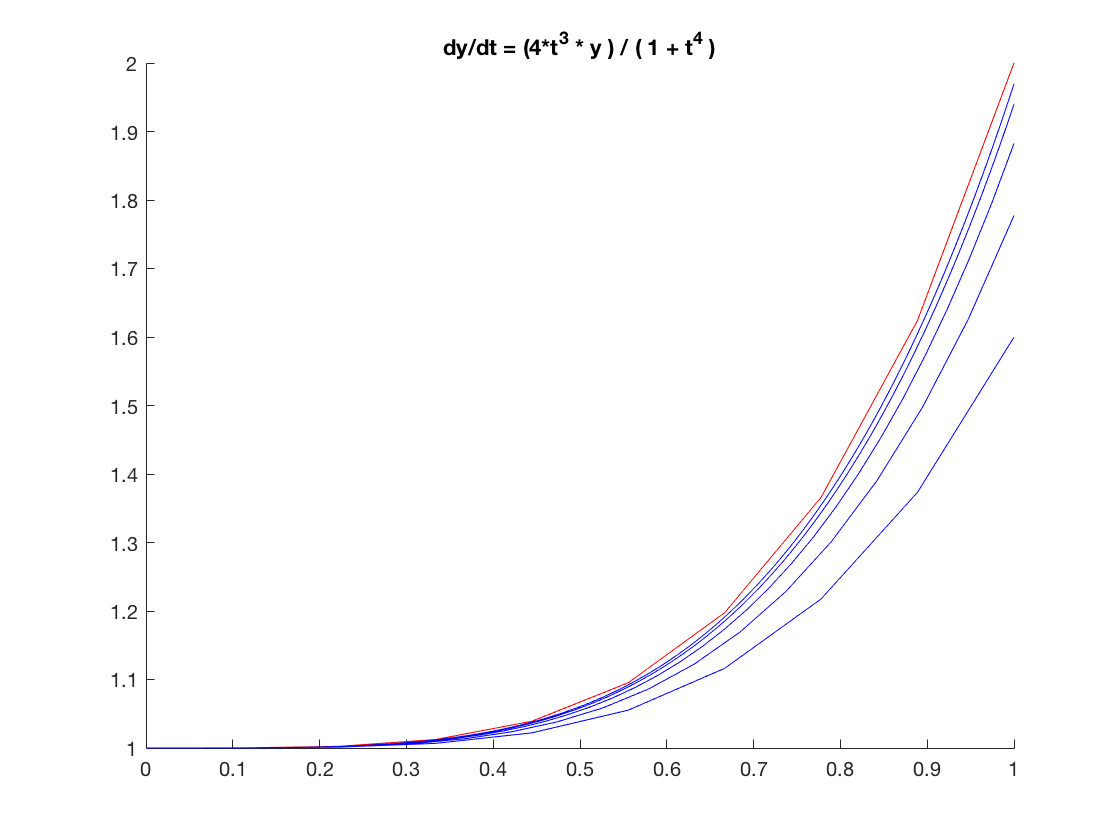
\includegraphics[height=8cm]{partc_4}\\
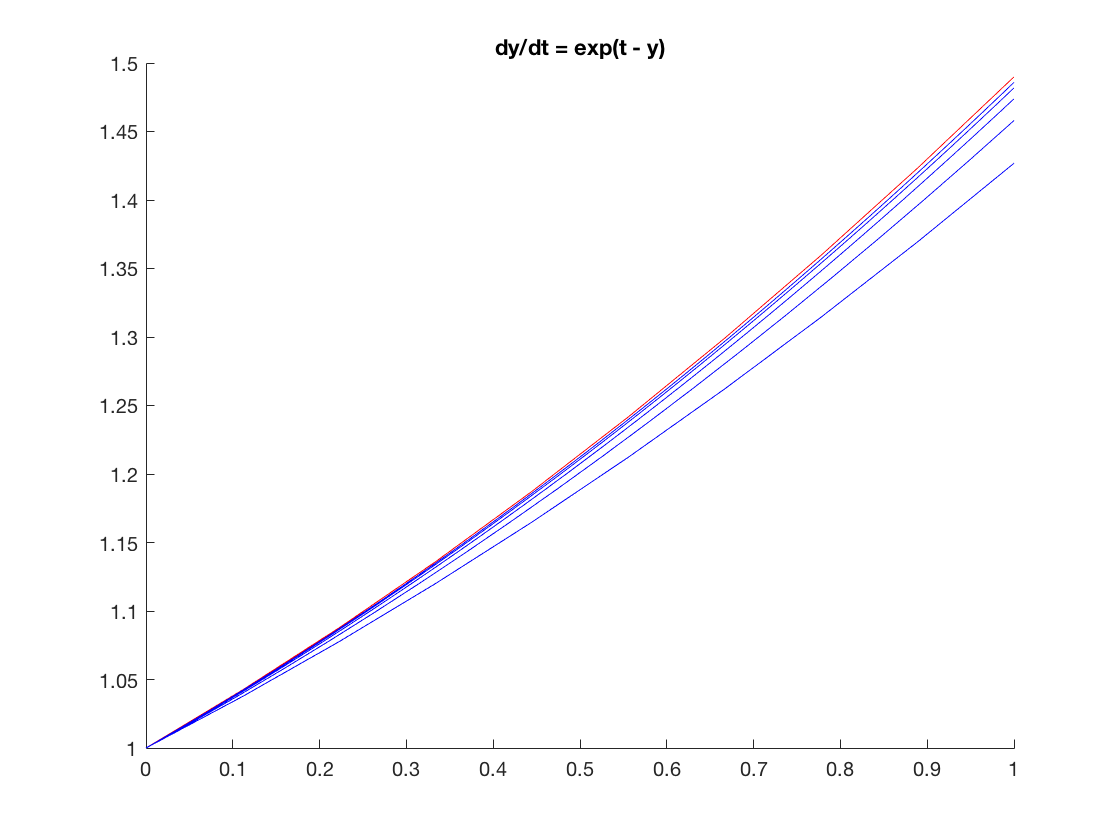
\includegraphics[height=8cm]{partc_5}\\
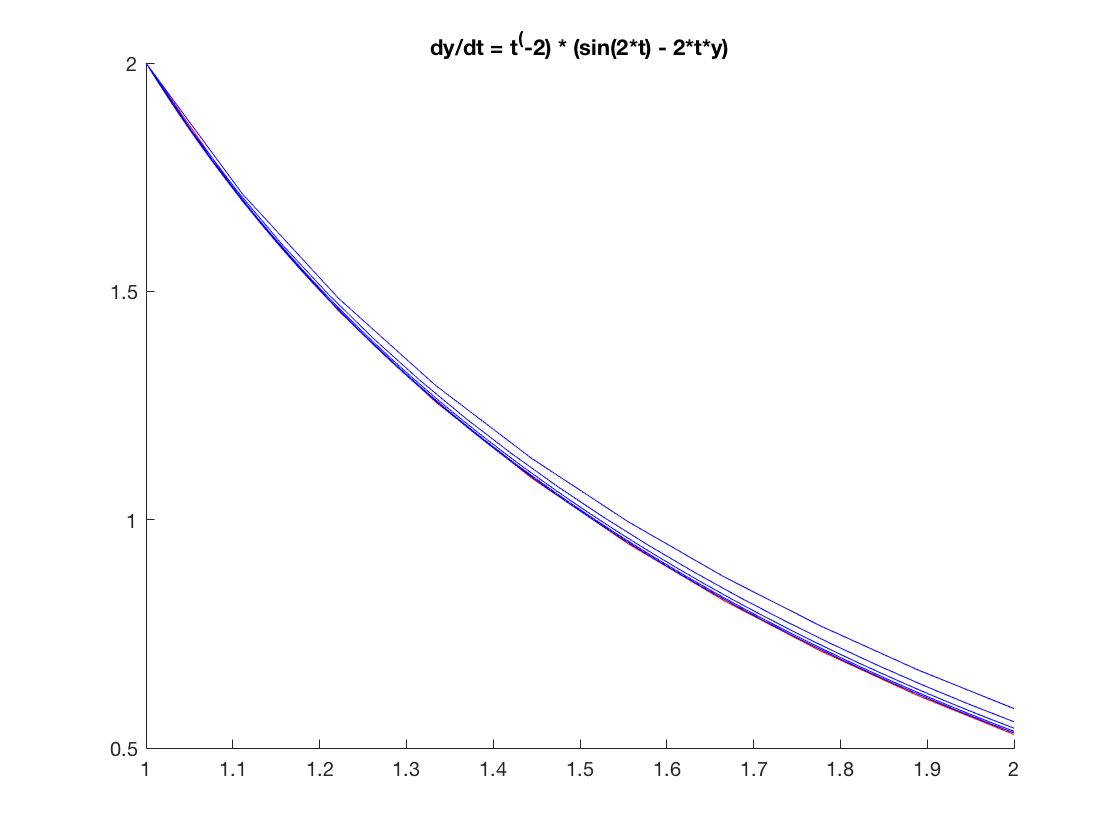
\includegraphics[height=8cm]{partc_6}\\
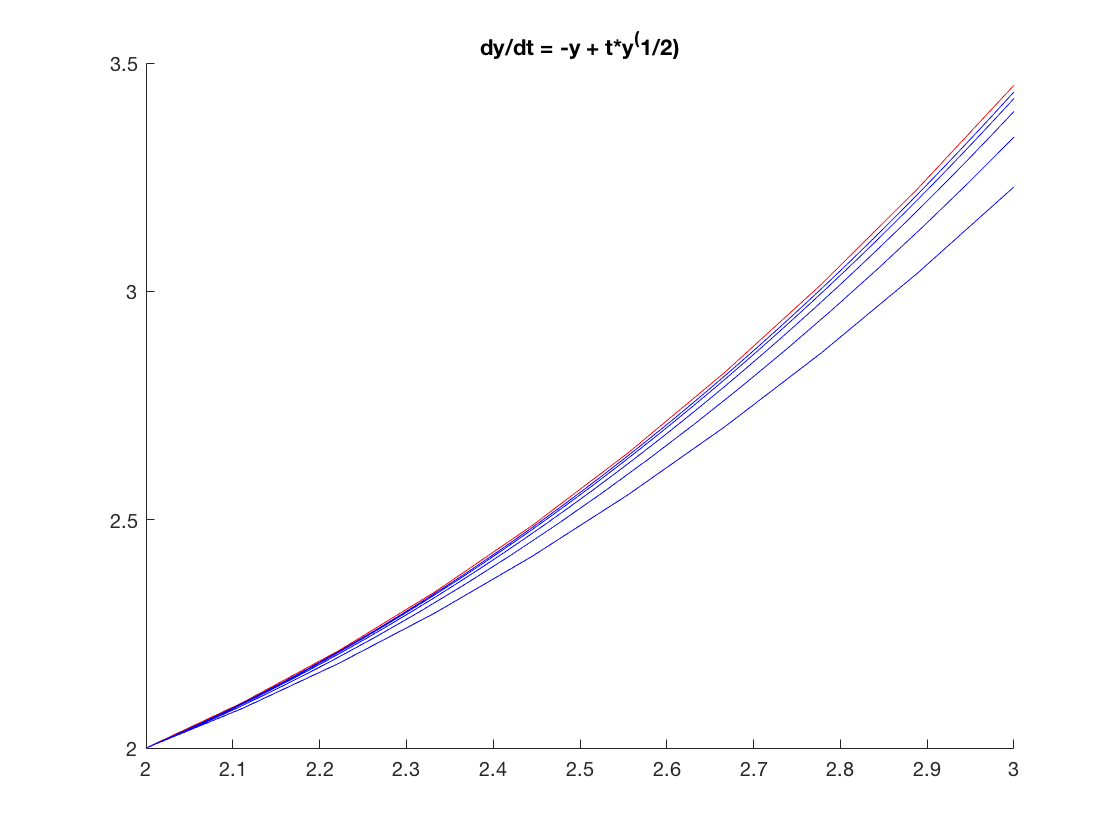
\includegraphics[height=8cm]{partc_7}\\

\subsection*{(e)}
All functions 5.1.1 a-d and 5.1.2 a-c satisfy the Lipschitz condition and have a unique unbounded unique solutions based on Theorem 2.4.1, 2.4.2, or 5.4. However, 5.1.2 d does not have an unbounded unique solution since it is undefined when $ty + t = 0$. 

\subsection*{(f)}
After experimenting with different bounds on 5.1.2 d and one can verify that different solutions exists on each one of those intervals. 

\section*{Part B}
In this section of the project we shall use a modified Ruga-Kutta to approximate solutions to systems of ordinary differential equations. 
\subsection*{(a)}
In order to accomplish this goal we need to modify the Ruga-Kutta function used in Part A to take in initial values of $y$'s as a vector. Then we have to issue that our calculations of the $k$'s also return a vector. Also when defining the problem one needs to remember that the function under investigation is not a vector function. 

\subsection*{(b)}
After modifying the Ruga-Kutta we tested it on the following system, 
$$ y′′ = −y, y(0)=0, y′(0)=1. $$
We obtained to the following graphs from running the method with a $T= 100$ and a $n=1000$. \\
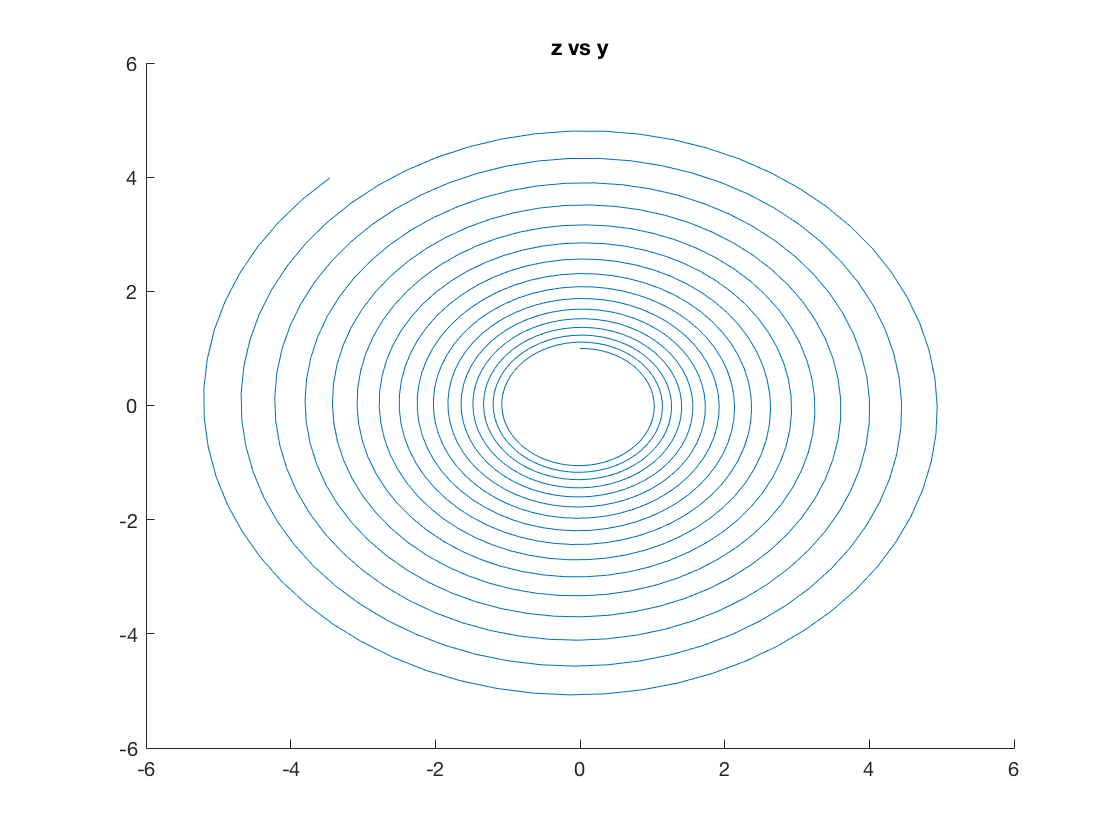
\includegraphics[height=8cm]{partB_1}\\
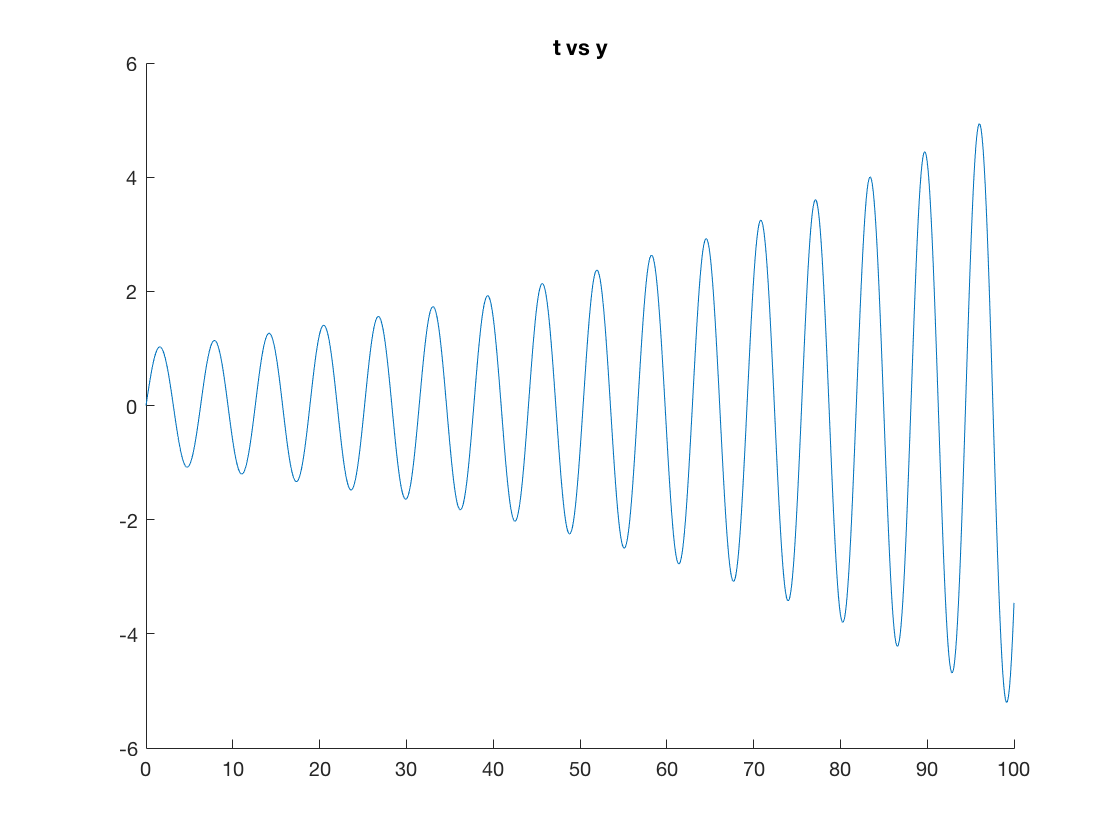
\includegraphics[height=8cm]{partB_2}\\

Also after experimenting with different values of $T$ and $n$, we made the following observation, (1) as $n$ increased the smoothness (less straight-lines) of the phase increased and (2) as the values of $T$ increased the scale of the solution increased as shown in the second graph.

\subsection*{(c)}
To further test the Ruga-Kutta we used the method on the following system, 
$$ y' = z$$
$$ z' = y (1 - y^2)$$
And we experimented with different initial conditions, after finding informative initial conditions we obtained the following pee-nut shaped graph. 

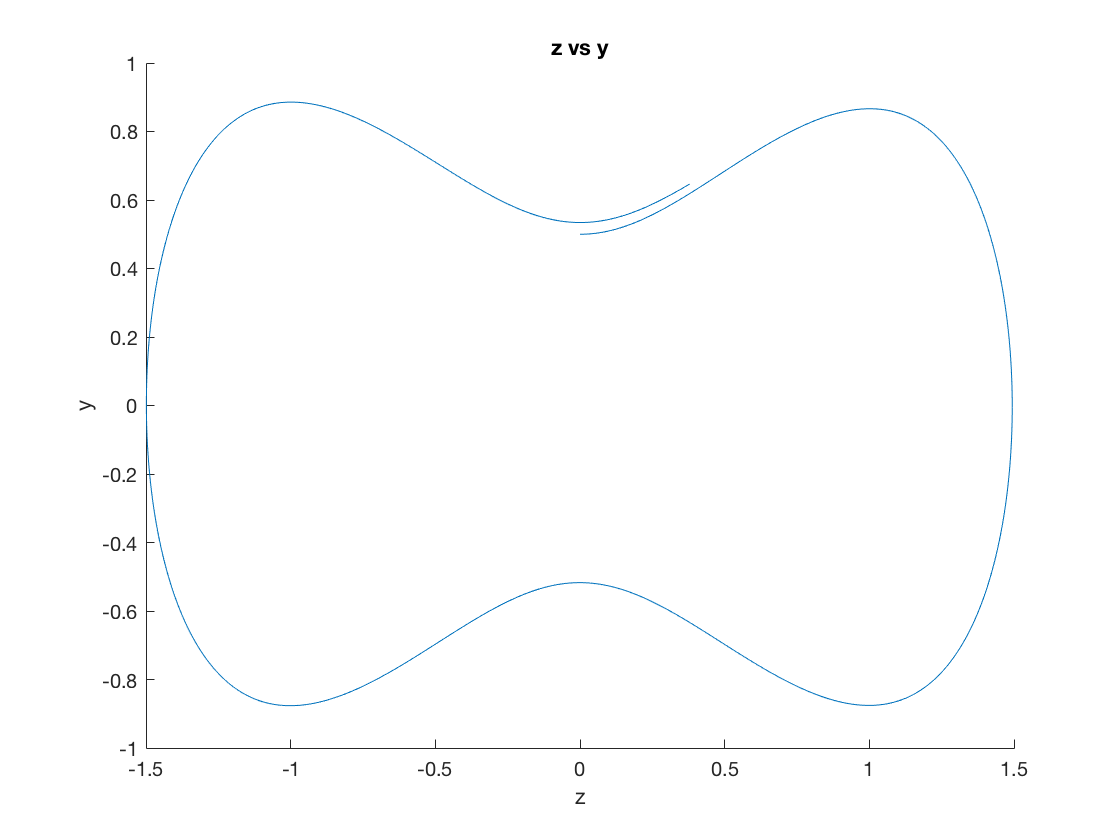
\includegraphics[height=8cm]{partB_3}\\

We can see from this figure that there is three equilibrium solutions at $z \in \{ -1,0,1 \} $ 

\subsection*{(d)}
The following figure was obtained after running the shooting method with $d \in \{ -1, -0.5, 0, 0.5, 1 \} $\\

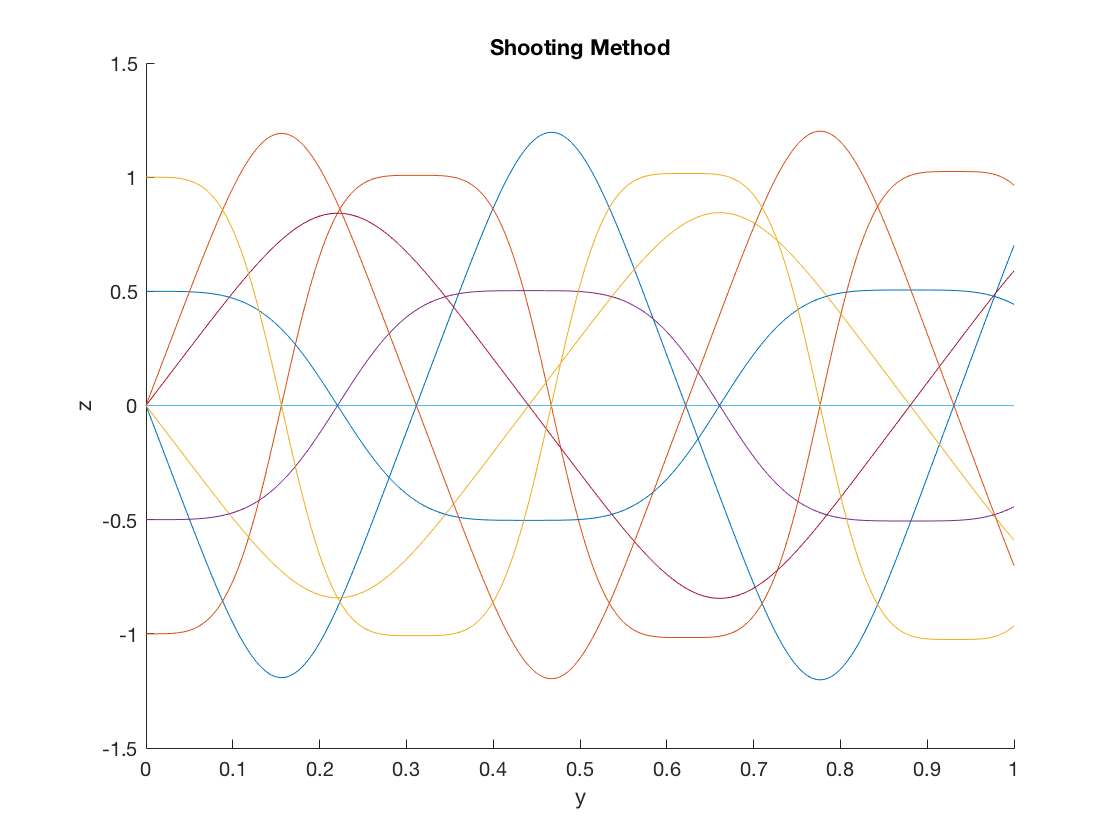
\includegraphics[height=8cm]{partB_4}\\


\end{document}
